\chapter{Especificaciones del robot delta seleccionado}\label{CAP5}
En este capítulo se presenta los valores de las dimensiones, masas e inercias que caracterizan el robot delta a simular. Se extraer los valores del prototipo del robot delta en tesis \cite{}, ya que en este documento no abarca la optimización dimensional de las piezas por energía y tampoco se tiene los límites de un espacio de trabajo determinado para una aplicación específica. La simplificación del robot delta se presenta en la siguiente figura:

    \begingroup
        \renewcommand{\arraystretch}{1.5}
        \begin{table}[H]
        \centering
        \begin{tabular}{c c{4cm} c}
           \hline
           \textbf{Parametro}  & \multicolumn{1}{c}{\textbf{Descripción}} & Valor \\\hline\hline
            $L_A$  & Longitud de un brazo           & 620 [mm]                        \\\hline
            $L_B$  & Longitud de un antebrazo       & 880 [mm]                         \\\hline
            $R_A$  & Radio de la Base fija           & 210 [mm]                         \\\hline
            $R_B$  & Radio de la plataforma móvil    & 50 [mm]                         \\\hline
            $m_a$  & Masa de un brazo                & 2.213 [kg]                         \\\hline
            $m_b$  & Masa de 1 varilla del antebrazo  & 657.5 [kg]                         \\\hline
            $m_c$  & Masa de la plataforma móvil     & 0.510 [kg]                         \\\hline
            $m_p$  & Masa de carga que es trasladada por el efector & 0 [kg]           \\\hline
            $m_{codo}$  & Masa de juntas que conectas los brazos con los antebrazos  & 0 [kg]  \\\hline
            $I_m$  & Inercia de los actuadores           &   0 [kg*m^2]     \\\hline
            $r_{masa}$  & Relación masas antebrazo           & 0.5        \\\hline
            $g$  & Gravedad           & 9.81  [m/s^2]                      \\\hline
        \end{tabular}
        \caption{Referencias del dibujo}
        \label{tab:cap5_tabla_1}
    \end{table}
    \endgroup
    
    \newpage
    
    
    \begin{figure}[htb]
        \centering
        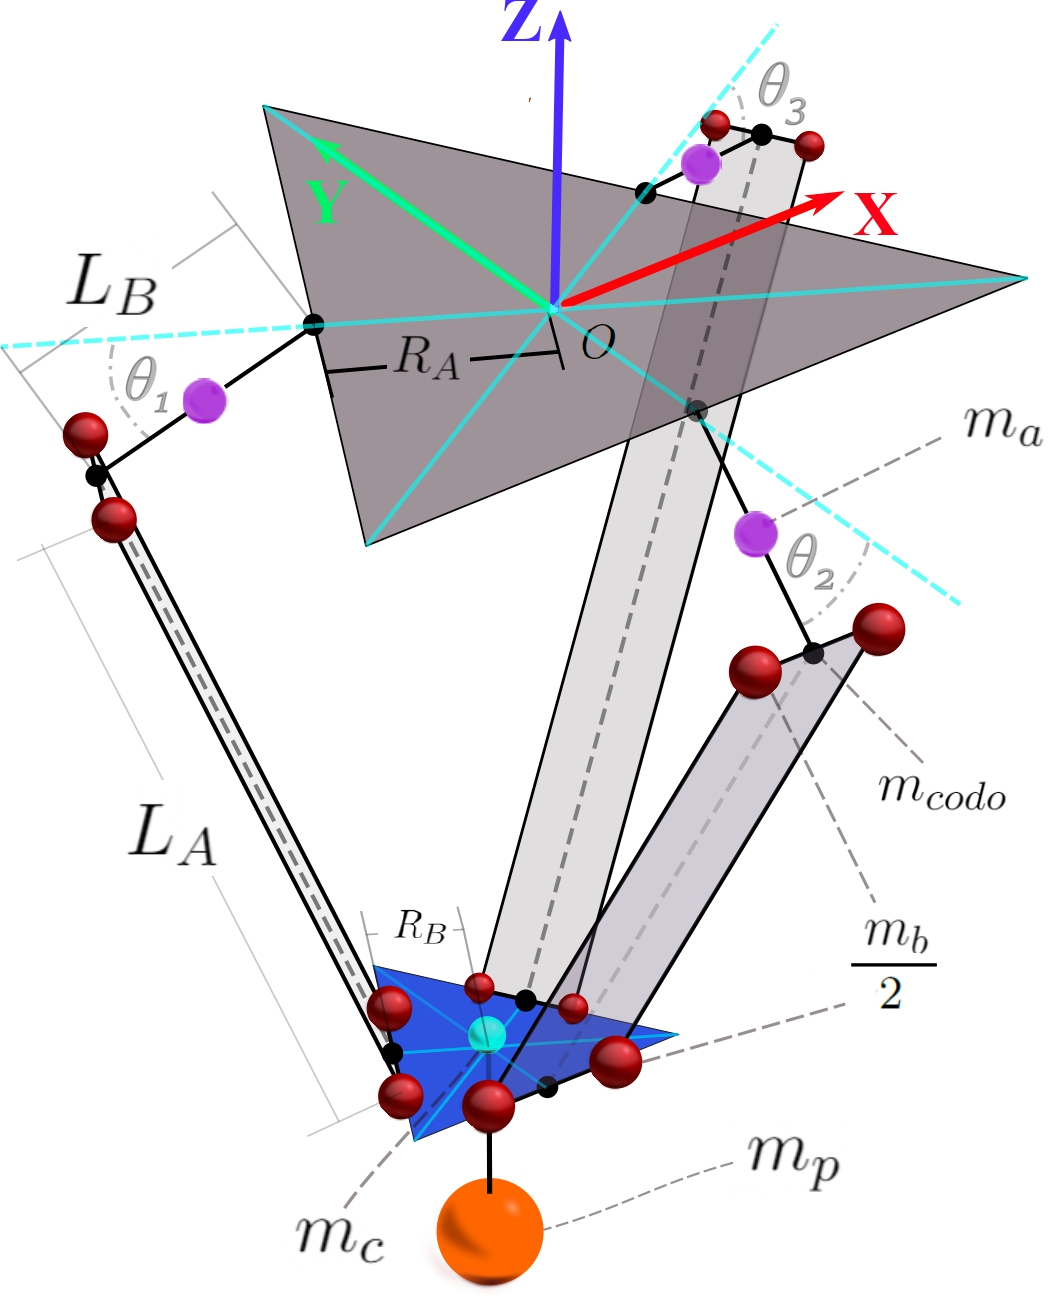
\includegraphics[width=1\linewidth]{Main/Chapter5/Images5/DIBUJO43.jpg}
        \caption{Caption}
        \label{fig:cap5_1}
    \end{figure}
    
    
    